\chapter{Manual Labour}
\pagestyle{fancy}
\label{ch:manual}

\fancyhf{} % here we clear any fancy header settings
%% Note, the first page of every chapter does not have a header.
\fancyhead[EC]{Linux System Administration}
\fancyhead[OC]{\leftmark} % O=odd pages, C= center, leftmark defaults to Chapter number and title
%\fancyhead[EC]{\rightmark} % E = even pages, C = center, rightmark defaults to number of current section
%%
%% Set, headheight to eliminate warning message "Package Fancyhdr Warning: \headheight is too small (12.0pt): Make it at least 13.59999pt.
\setlength{\headheight}{13.6pt} 
%%\setlength{\footheight}{13.6pt}
%%
% The next line would put a line at the bottom of every page starting from the second page of every chapter, if it was uncommented.
%%
%\renewcommand{\footrulewidth}{1pt}
%%
\cfoot{\thepage} % c = center, foot = footer, thepage = page number

\rhead{
\includegraphics[width=.5cm]{figures/smCanadianFlag}}

		
%%%%%%%%%%%%%%%%%%%%%%%%%%%%%%%%%%%%%%%%%%%%%%%%%%%%%%%%%%%
%%%%%%%%%%%%%%%%%%%%%%%%%%%%%%%%%%%%%%%%%%%%%%%%%%%%%%%%%%%
\section{Introduction}
There is such an abundance of help available to learn Linux. Firstly,  \keyword{manpages} are the text-based help system that is available at the command line.  To access a \emph{manpage}, you simple type \tbi{man} \emph{command}. You, of course, need to know the name of the \emph{command}. All manpages have section headers that separate the information into categories. Here are some examples of the manpage headings for two commands: \keyword{tar} and \keyword{ps}. I will not display the contents of the actual manpage. pohtatoes, paTatoe, man page, man-page, manpage, there seems to be no one standard as to how to spell this...I will use only manpage.

\begin{lstlisting}[escapeinside={¿}{¿},frame=single,breaklines]
#
# Here are the headers for the tar command.
#
¿\tld¿ man tar | grep '^[A-Z]'
TAR(1)                                            GNU TAR Manual                                            TAR(1)
NAME
SYNOPSIS
NOTE
DESCRIPTION
OPTIONS
RETURN VALUE
SEE ALSO
BUG REPORTS
COPYRIGHT
TAR                                              February 22, 2014                                          TAR(1)
#
# And, for the ps command.
#
¿\tld¿ man ps | grep '^[A-Z]'
PS(1)                                              User Commands                                             PS(1)
NAME
SYNOPSIS
DESCRIPTION
EXAMPLES
SIMPLE PROCESS SELECTION
PROCESS SELECTION BY LIST
OUTPUT FORMAT CONTROL
OUTPUT MODIFIERS
THREAD DISPLAY
OTHER INFORMATION
NOTES
PROCESS FLAGS
PROCESS STATE CODES
OBSOLETE SORT KEYS
AIX FORMAT DESCRIPTORS
STANDARD FORMAT SPECIFIERS
ENVIRONMENT VARIABLES
PERSONALITY
SEE ALSO
STANDARDS
AUTHOR
\end{lstlisting}

Even though the information will have some common section headers, the information will vary somewhat according to the energy and documentation skills of the maintainer of the manpage...and according to the complexity of the command.\\

\section{Resources on the Internet}

You can also find \keyword{manpages} on the Internet. Here is a list of some of the top webpages that present their information in the \tbi{manpage} format.

\begin{itemize}
	\item \tbi{\href{https://www.gnu.org/manual/manual.html}{GNU Manuals Online }}Official GNU packages with their primary documentation.
	\item \tbi {\href{http://linuxmanpages.net/index.html}{fedora manuals }}Manpages extracted from the official Fedora RPMs.
	\item \tbi{\href{https://www.kernel.org/doc/man-pages/}{The Linux man-pages project} }Documents the Linux kernel and C library interfaces employed by user-space programs. Linux Manual Pages from \href{http://www.tldp.org/manpages/man.html}{The Linux Documentation Project}.
	\item \tbi{\href{http://man7.org/linux/man-pages/index.html}{Linux man pages online }}HTML renderings of the man pages from the Linux man-pages project.
	\item \tbi{\href{http://linuxcommand.org/superman_pages.php}{SuperMan pages }} Deprecated, but still useful version of man pages, from \href{http://linuxcommand.org/}{LinuxCommand.org}.
	\item \tbi{\href{man.cx}{Manpages }}  A catchall for manpages that you just can't find online or onhost.	
\end{itemize}

\section{How not to grep manpages}

Am I am a huge fan of the Linux manpages? Oh, yeah! When I am trying to figure something out, I begin by reading the man page. The more I work with Linux, the more familiar I become with the content of the manpages. But, the more I worked with manpages, the more I became aware of the deficiencies of manpages. So, How not to grep manpages? I will be illustrating a process of discovery (mine), as I find a more logical way of grepping manpages.

\begin{tabularx}{\linewidth}{X | X} % the X is needed to wrap text
\caption{Manpages}\label{table:manpages-comparison}\\ % title of Table
\toprule
Pros & Cons \\% inserts table heading, unbolds 1st column heading
\midrule
Provides a quick reference. & Not meant as a tutorial, it is assumed that you have some basic understanding of the command and its configuration.\\[2mm]
All info in one document. & You have to page through multiple screens of information.\\[2mm]
Information is organized into logical sections. & Manpages vary in quality and are quite terse.\\[2mm]
Format is similar, options and keywords are listed. & Keywords are not highlighted, no colouring, and may appear in random order.\\[2mm]
Information is searchable using patterns. & Syntax is complex and the information that is returned may not be what you are looking for.\\[2mm]
You can search all manpages at once for keywords. & You must filter your seaches in order to isolate relevant information.\\[2mm]
Fairly simple and easy-to-use. & Format is based on a 2001 technical standard and thus do not include common features such as hyperlinks.\\[2mm]
Command options are listed with explanations. & Options and examples may be difficult to locate within manpage.\\[2mm]
\bottomrule
\end{tabularx}

The following code will help you more efficiently grep specific sections of a manpage. Please read the comments carefully as I take a while to arrive at the correct way to grep a manpage.

\begin{lstlisting}[escapeinside={¿}{¿},frame=single,breaklines]
#
# I want to start reading a manpage. manpages are displayed a screen at a time, hit the  spacebar or 'Page Down' buttons to advance the manpage a screen or the down arrow to advance one line. Similarily, 'Page Up' goes back one screen and the up arrow goes back one line. Press q to quit the manpage.
#
¿\tld¿ man ps
#
#
# But, this would provide the whole manpage. Suppose, I just wanted to get all lines that begin with the string "Select".
#
¿\tld¿ grep "Select" man ps
grep: man: No such file or directory
grep: ps: No such file or directory
#
# Oh yeah, grep thinks that man and ps are file names. But, surrounding 'man ps' with single quotes does not make sense given that 'man ps' is not a file name (a string), it is a command with an argument. Maybe we have to use command substitution? Note, I am using backquotes ` for command substitution, not single vertical quotes '.
# 
¿\tld¿ grep "Select" `man ps`
grep: invalid option -- ¿\tqs{"}¿
Usage: grep [OPTION]... PATTERN [FILE]...
Try 'grep --help' for more information.
#
# Hmm, well that didn't work! And, here begins an example of how one can arrive at a solution learning all along the way. You may often find that your initial solution is wonky and that a more efficient solution is available. Hint, hint!
#
# So, ¿\textbf{\color{red}initially}¿, I decide that the only way that one could grep a man page was to first send the manpage to a file and then grep the file. I first pipe the man page to 'col -b' to format the file properly. 
#
¿\textbf{\color{red}For experienced Linux users, be patient! I will get to the correct way of grepping a manpage, so read on.}¿
#
# I am writing two independent commands on the next line. The commands are separated by the command separator, the semi-colon. The first command creates the file 'ps.man'. The second command greps "Select" from this file.
#
¿\tld¿ man ps | col -b > ps.man ; grep "Select" ps.man
-A     Select all processes.  Identical to -e.
-a     Select all processes except both session leaders (see getsid(2)) and processes not associated
.
.
Select by command name.  This selects the processes whose executable name is given in cmdlist.
.
.
Select by effective user ID (EUID) or name.  Identical to -u and U.
#
# Ok, that worked...mostly. I elided several lines (indicated by the two vertical periods because the output was quite long). But, notice that there were many lines that just began with the string "Select". We don't know anything about the context of the line. Is there an option associated with this line? Because I am familiar with the structure of the manpages, I knew I had to use the before and after grep options for the lines that begin with "Select". Actually, these lines begin with spaces. To summarise, I want lines above and below the lines containing "Select". I therefore use grep's -C switch (number of context lines around the line). Note: The leading spaces in the actual manpage are truncated when the selection is sent to the command line.
#
# -E = we need the power of regex
# -C3 = 3 lines of context above and below the string
# "\ *Select" = search for lines that begin with any number of spaces followed by the string "Select"
#
¿\tld¿ grep -E -C3  "\ *Select" ps.man
selected by other means.	An alternate description is that this option causes ps to list all
processes with a terminal (tty), or to list all processes when used together with the x option.

-A     Select all processes.  Identical to -e.

-a     Select all processes except both session leaders (see getsid(2)) and processes not associated with a terminal.
.
.
-C cmdlist
Select by command name.  This selects the processes whose executable name is given in cmdlist.
.
.
--User userlist
Select by real user ID (RUID) or name.  Identical to -U.

--user userlist
Select by effective user ID (EUID) or name.  Identical to -u and U.
#
# Ok, that worked better. I have more useful information about each item.
#
# How about another diversion? A diversion within a diversion. What's that called? 
#
# How about a different use of grep? Let's say I just want to see the explanation of the -f option for the ps command. Note: I don't use the exact option for grep, so lines beginning with --format, --forest, -F are also returned.
#
¿\tld¿ grep -E "\ *-f" ps.man
	-f     Do full-format listing. This option can be combined with many other UNIX-style options to add
	-F     Extra full format.  See the -f option, which -F implies.
	--format format
		Specify user-defined format.  Identical to -o and --format.
		the -f format option and with the various BSD-style format options, which all normally display the command arguments.  See the -f option, the format keyword args, and the format keyword comm.
	--forest
			keyword, the -f option, and the c option.
			ucmd, ucomm).  See also the args format keyword, the -f option, and the c option.
#
# Is there another way of getting this information? The following will also dump the exact same information.
#
¿\tld¿ grep -E \\-f ps.man
#
# In a subsequent section, you will see that we use a variation of the above command to grep a manpage directly.
#
\end{lstlisting}

I can add a function to my \textsl{.bashrc} file that creates \textsl{manpagename.man} files. When I wanted to grep a manpage, I grep instead the \textsl{manpagename.man} file. Here is the function:

\begin{lstlisting}[escapeinside={¿}{¿},frame=single,breaklines]
function manup ()
{
man $1 | col -b > $1.man
}
\end{lstlisting}

Here is an example of how you could use the function. Since the command itself is a little cumbersome, I also considered creating a another function that would call a function using parameters. Go ahead and try creating that function. My philosophy is: \textit{If you use a complex command repeatedly, simplify it by creating a \emph{.bashrc} alias or function}.

\begin{lstlisting}[escapeinside={¿}{¿},frame=single,breaklines]
¿\tld¿ manup ls
¿\tld¿ grep -E -C1 "\ *--inode" ls.man
-i, --inode
print the index number of each file
\end{lstlisting}

Now, here's the \tbi{about face}, or maybe, the \tbi{saving face}. In a comment section above, I used the adverb \emph{initally} and asked that experienced users be patient. My command didn't work when I put \keyword{grep} before the command. I had the command order backwards. I needed to \emph{man} and then \emph{grep}.

\begin{lstlisting}[escapeinside={¿}{¿},frame=single,breaklines]
#
# Before we begin, an aside...what would happen if you issued the following command? Note the pipe symbol.
#
¿\tld¿ grep "Select" | man ps
#
# The ps manpage would open. q for quit would work only if you paged down to the bottom.
#
# We also saw that when we issued the followign command, we got errors...
#
¿\tld¿ grep "Select" `man ps`
grep: invalid option -- ¿\tqs{"}¿
Usage: grep [OPTION]... PATTERN [FILE]...
Try 'grep --help' for more information.
# 
# Brain, turn thyself on!. Let's reverse the order of the commands. As you can see, we need to pipe the manpage to the grep command. As I said previously, the grep command is powerful, but you need to experiment to get things right.
#
¿\tld¿ man ps | grep Select
-A     Select all processes.  Identical to -e.
.
.
Select by effective user ID (EUID) or name.  Identical to -u and U.
#
# I am only showing the first and last lines of the output. As you see, when we grepped, we lost the context of the last line. We still need to use grep's context option.
#
¿\tld¿ man ps | grep -C 3 Select
-A     Select all processes.  Identical to -e.
.
.
--user userlist
Select by effective user ID (EUID) or name.  Identical to -u and U.
\end{lstlisting}

\section{Finding manages}

Finding all \keyword{manpages} related to a specific command is not as straightforward as it should be. I will work through a few examples below and then summarise the commands in a table. There are two commands that we use to search for manpages: \tbi{man} and \tbi{apropos}. We are going to use the \tbi{stat} command to explore this topic.

\begin{lstlisting}[escapeinside={¿}{¿},frame=single,breaklines]
#
# Ok, let's begin by searching for manpages that relate to the stat command.  Note, the 'man -k stat' command will list all manpages that include the string ¿\textbf{\color{red}stat}¿ which may appear as part of the actual manpage name or as part of the description of the manpage. I will also get a count for each search.
#
#
¿\tld¿ man -k stat ; man -k stat | wc -l
XML::XPath (3pm)     - a set of modules for parsing and evaluating XPath ¿\textbf{\color{red}stat}¿ements
ac (1)               - print ¿\textbf{\color{red}stat}¿istics about users' connect time
aio_error (3)        - get error ¿\textbf{\color{red}stat}¿us of asynchronous I/O operation
.
.
App::Prove::¿\textbf{\color{red}Stat}¿e (3pm) - ¿\textbf{\color{red}Stat}¿e storage for the "prove" command.
.
.
Xutf8ResetIC (3)     - reset the ¿\textbf{\color{red}stat}¿e of an input context
XwcResetIC (3)       - reset the ¿\textbf{\color{red}stat}¿e of an input context
347
#
# Whoa, way too much information, there are 347 lines of information. We need to filter our search to exclude commands that have nothing to do with the stat command. Several commands not related to the stat command made the list just because their description include the string "stat" such as the command XwcResetIC whose description says: reset the ¿\textbf{\color{red}stat}¿e of an input context.
#
# Alright, so we need the string "stat" when it begins the line. Therefore, we use the circumflex which signifies "start of a line". We see below that our list is now only 15 items long.
#
¿\tld¿ man -k '^stat' ; man -k '^stat' | wc -l
App::Prove::State (3pm) - State storage for the "prove" command.
fstab (5)            - static information about the filesystems
hosts (5)            - static table lookup for hostnames
iftab (5)            - static information about the network interfaces
ip-monitor (8)       - state monitoring
stat (1)             - display file or file system status
stat (2)             - get file status
stat (3p)            - get file status
stat64 (2)           - get file status
statd (8)            - NSM service daemon
statfs (2)           - get filesystem statistics
statfs64 (2)         - get filesystem statistics
statvfs (2)          - get filesystem statistics
statvfs (3)          - get filesystem statistics
statvfs (3p)         - get file system information
15
#
# Well, that's better, but we still have lines whose description begins with ¿\textbf{\color{red}stat}¿e. So, 'man -k '^stat' seems to be applied on two columns, the command column and the description column. We obviously need to say only the string itself, note the string as part of a larger string. We therefore can use grep's block option.
#
¿\tld¿ man -k '^stat' | grep '\bstat\b'
stat (1)             - display file or file system status
stat (2)             - get file status
stat (3p)            - get file status
#
# We can also use grep's word option.
#
¿\tld¿ man -k '^stat' | grep -w stat
stat (1)             - display file or file system status
stat (2)             - get file status
stat (3p)            - get file status
#
# Ok, now we see that stat has three relevant man pages. But, as always with Linux there is usually more than one way to get this information.
#
¿\tld¿ whatis whatis
whatis (1)           - display one-line manual page descriptions

¿\tld¿ whatis stat
stat (2)             - get file status
stat (3p)            - get file status
stat (1)             - display file or file system statusw
#
# We can also get this list with the man -f option, --whatis.
#
¿\tld¿ man -f stat
stat (2)             - get file status
stat (3p)            - get file status
stat (1)             - display file or file system status
\end{lstlisting}

\section{What are manpages?}

Now that we know how to search for all \keyword{manpages} related to a command, let's dig a bit deeper into the content of manpages. I am going to use my \emph{mang} function to get just the \tbi{man} \emph{manpage} \small{DESCRIPTION} section. This listing from the \tbi{man} \emph{manpage} answers the question posed in the section title: What are manpages?

\begin{lstlisting}[escapeinside={¿}{¿},frame=single,breaklines]
¿\tld¿ mang man description examples
DESCRIPTION
man is the system's manual pager.  Each page argument given to man is normally the name of a program, utility or function. The manual page associated with each of these arguments is then found and  displayed. A section, if provided, will direct man to look only in that section of the manual.  The default action is to search in all of the available sections following a pre-defined order ("1 1p 8 2 3 3p 4 5 6 7 9 0p n l p o 1x  2x  3x 4x 5x 6x 7x 8x" by default, unless overridden by the SECTION directive in /etc/man_db.conf), and to show only the first page found, even if page exists in several sections.

The table below shows the section numbers of the manual followed by the types of pages they contain.

1   Executable programs or shell commands
2   System calls (functions provided by the kernel)
3   Library calls (functions within program libraries)
4   Special files (usually found in /dev)
5   File formats and conventions eg /etc/passwd
6   Games
7   Miscellaneous (including macro packages and conventions), e.g. man(7), groff(7)
8   System administration commands (usually only for root)
9   Kernel routines [Non standard]

A manual page consists of several sections.

Conventional section names  include  NAME,  SYNOPSIS,  CONFIGURATION,  DESCRIPTION,  OPTIONS,  EXIT STATUS, RETURN VALUE,  ERRORS,  ENVIRONMENT,  FILES,  VERSIONS,	CONFORMING TO,	NOTES, BUGS, EXAMPLE, AUTHORS, and SEE ALSO.

The following conventions apply to the SYNOPSIS section and can be used as a guide in other sections.

bold text	  type exactly as shown.
italic text	  replace with appropriate argument.
[-abc]		  any or all arguments within [ ] are optional.
-a|-b		  options delimited by | cannot be used together.
argument ...	  argument is repeatable.
[expression] ...	  entire expression within [ ] is repeatable.

Exact rendering may vary depending on the output device. For instance, man will usually	 not  be  able to render italics when running in a terminal, and will typically use underlined or coloured text instead.

The  command  or function  illustration	 is a pattern that should match all possible invocations.  In some cases it is advisable to illustrate several exclusive invocations as is shown in the  SYNOPSIS  section	of this manual page.
\end{lstlisting}

\section{Where are manpages stored?}

\begin{lstlisting}[escapeinside={¿}{¿},frame=single,breaklines]
¿\tld¿ whereis man
man: /usr/bin/man /usr/share/man /usr/share/man/man7/man.7.gz /usr/share/man/man1/man.1.gz /usr/share/man/man1p/man.1p.gz
\end{lstlisting}

\section{What type of file is the man command and why is it hashed?}

\begin{lstlisting}[escapeinside={¿}{¿},frame=single,breaklines]
¿\tld¿ type man
man is hashed (/usr/bin/man)

¿\tld¿ type hash
hash is a shell builtin
#
# Say what? Let's use my mbib function to get some info on hash from the 'man builtin' manpage..
#
¿\tld¿ mbib hash help
hash [-lr] [-p filename] [-dt] [name]
Each time hash is invoked, the full pathname of the command name	is  determined	by  searching  the directories  in  $PATH  and remembered.  Any previously-remembered pathname is discarded.	 If the -p option is supplied, no path search is performed, and filename is used as the full	filename  of  the command. The  -r option causes the shell to forget all remembered locations.  The -d option causes the shell to forget the remembered location of each name.	 If the -t option is  supplied,	 the  full pathname	to  which  each name corresponds is printed.  If multiple name arguments are supplied with -t, the name is printed before the hashed full pathname.	The -l option causes  output  to  be  displayed  in  a  format that may be reused as input.  If no arguments are given, or if only -l is supplied, information about remembered commands is printed.	The return status is true unless a name is not found or an invalid option is supplied.
#
# Let's get some info from the bash manpage.
#
¿\tld¿ man bash | grep -A15 -i '^command execution$'
COMMAND EXECUTION
After a command has been split into words, if it results in a simple command and an optional list of arguments, the following actions are taken.

If the command name contains no slashes, the shell attempts to locate it.  If there exists a shell function by  that  name, that function is invoked as described above in FUNCTIONS.  If the name does not match a function, the shell searches for it in the list of shell builtins.  If a match is found, that builtin is invoked.

If the name is neither a shell function nor a builtin, and contains no slashes, bash searches each element of the PATH  for a  directory  containing  an  executable  file by that name.  Bash uses a hash table to remember the full pathnames of executable files (see hash under SHELL BUILTIN COMMANDS below).  A full search of the directories in PATH is performed only if the command is not found in the hash table.  If the search is unsuccessful, the shell searches for a defined shell function named command_not_found_handle.  If that function exists, it is invoked with the original command  and  the  original  command's  arguments  as its arguments, and the function's exit status becomes the exit status of the shell.  If that function is not defined, the shell prints an error message and returns an exit status of 127.

¿\tld¿ man bash | grep -A3 'BASH_CMDS'
BASH_CMDS
An  associative  array variable whose members correspond to the internal hash table of commands as maintained by the hash builtin.  Elements added to this array appear in the hash table; unsetting array elements cause commands to  be removed from the hash table.
#
# What is in our hash table?
#
¿\tld¿ hash -l
builtin hash -p /usr/bin/grep grep
builtin hash -p /usr/bin/vim vim
builtin hash -p /usr/bin/man man
builtin hash -p /usr/bin/info info
builtin hash -p /usr/bin/ls ls
#
# What about some other commands?
# 
¿\tld¿ type awk
awk is /usr/bin/awk

¿\tld¿ type alias
alias is a shell builtin
#
# But, notice that our alias overrides the hash state of the ls command.
#
¿\tld¿ type ls
ls is aliased to `ls --color=auto'

\end{lstlisting}

\section{Calling manpages}

Ok, so we know how to get a list of all man pages for a command. Note, in our list of the \keyword{stat} man pages that \emph{stat} was followed by an index number of some sort. Take a look at the \small{DESCRIPTION} section of the \tbi{man} \emph{manpage}.  The author of the \tbi{man} \emph{manpage} twice used the word \tbi{section}, once to describe \emph{the types of manpages} and again as \emph{conventional section names}. I humbly suggest that this leads to some confusion. Here are exerts from the \tbi{man} \emph{manpage}...

\begin{enumerate}
	\item{The table below shows the \tbi{section} numbers of the manual followed by the types of pages they contain.}\\
	The \tbi{man} \emph{manpage} author then gives a numbered list describing these \tbi{sections}.
	\item{A manual page consists of several \tbi{sections.}}\\
	The \tbi{man} \emph{manpage} author then gives a unordered list of \tbi{Conventional section names.}
\end{enumerate}

My contention is that he should have said \tbi{manpage index numbers} for the first and \tbi{manpage section headers} for the second. I call the different manpages with \tbi{manpage index numbers} and filter manpage information using \tbi{manpage section headers}. Although there is a \keyword{man} option \tqs{-S, -s, -{}-{}sections=LIST}, it is optional to use. You open the manpage by calling the manpage preceded by its \tbi{manpage index number}.

\begin{lstlisting}[escapeinside={¿}{¿},frame=single,breaklines]
#
# List the 'man page index numbers' for the stat command...shown in red. Note, the default section number is 1. Calling a man page without specifying a section number defaults to this index number.
#
¿\tld¿ man -f stat
stat ¿\color{red}{(2)}¿            - get file status
stat ¿\color{red}{(3p)}¿            - get file status
stat ¿\color{red}{(1)}¿             - display file or file system status
#
# Open a manpage by referencing the 'manpage index number'. I do not show the actual man page. Note, the -S option is optional, we can just open this man page with 'man 3p stat'.
#
¿\tld¿ man -S 3p stat
#
# Ok, let's get the description for each of the three stat manpages combining the insight gained above.
#
¿\tld¿ man 1 stat | grep -A1 -x DESCRIPTION
DESCRIPTION
Display file or file system status.

¿\tld¿ man 2 stat | grep -A3 -x DESCRIPTION
DESCRIPTION
These  functions  return  information  about  a file, in the buffer pointed to by stat.  No permissions are required on the file itself, but—in the case of stat(), fstatat(), and lstat()—execute (search)  permission is required on all of the directories in pathname that lead to the file.

¿\tld¿ man 3p stat | grep -A3 -x DESCRIPTION
DESCRIPTION
Refer to fstatat().
#
# Conclusion: We call manpages by their manpage index numbers, with the manpage index number preceeding the actual manpage name. As well, I can grep manpage section headers when searching information within a manpage.
#
\end{lstlisting}

\section{Searching manpages with apropos}

We can also search for material within manpages by using the \keyword{aprops} command. When you don't know how to procede at the command line, start with \emph{apropos}.

\begin{lstlisting}[escapeinside={¿}{¿},frame=single,breaklines]
#
# What is apropos?
#
¿\tld¿ whatis apropos
apropos (1)          - search the manual page names and descriptions
#
# Does man have an option like the --whatis option? Of course, it does!
#
¿\tld¿ man --help | grep apropos
-k, --apropos              equivalent to apropos
-K, --global-apropos       search for text in all pages
#
# Let's see what the DESCRIPITON section of the apropos man page says.
#
¿\tld¿ man apropos | grep -A2 -x DESCRIPTION
DESCRIPTION
Each  manual  page  has  a  short  description  available within it.  apropos searches the descriptions for instances of keyword.
#
# What is stat?
#
¿\tld¿ whatis stat
stat (2)             - get file status
stat (3p)            - get file status
stat (1)             - display file or file system status
#
# Instead of searching for the command name stat, let's search manpages for status. Note, we get a list with 98 items.
#
¿\tld¿ apropos status
aio_error (3)        - get error status of asynchronous I/O operation
aio_error (3p)       - retrieve errors status for an asynchronous I/O operation
aio_return (3)       - get return status of asynchronous I/O operation
.
.
X509_verify_cert_error_string (3ssl) - get or set certificate verification status information
XkbGetDeviceInfo (3) - Determine whether the X server allows Xkb access to particular capabilities of input device...

¿\tld¿ apropos status | wc -l
98
#
# Let's narrow this down...and focus on the command stat.
#
¿\tld¿ apropos status | grep '^stat'
stat (1)             - display file or file system status
stat (2)             - get file status
stat (3p)            - get file status
stat64 (2)           - get file status
#
# Hey, we found stat64 again! Remember, from above when we grepped on the block stat, stat64 fell off our list. 
#
# Let's repeat the above but, use apropos to find stat. Howe many pages does it find?
#
¿\tld¿ apropos stat | wc -l
347
#
# Ok, let's narrow it down...
#
¿\tld¿ apropos stat | grep '^stat'
stat (1)             - display file or file system status
stat (2)             - get file status
stat (3p)            - get file status
stat64 (2)           - get file status
statd (8)            - NSM service daemon
statfs (2)           - get filesystem statistics
statfs64 (2)         - get filesystem statistics
statvfs (2)          - get filesystem statistics
statvfs (3)          - get filesystem statistics
statvfs (3p)         - get file system information
#
Are man pages actual files? It turns out that they are and they are compressed files.
#
¿\tld¿ man -aw stat
/usr/share/man/man1/stat.1.gz
/usr/share/man/man2/stat.2.gz
/usr/share/man/man3p/stat.3p.gz
#
# We can even open the manpage by opening its actual manpage file. I will not actually display the manpage.
#
¿\tld¿ man /usr/share/man/man3p/stat.3p.gz
#
# Let's try with a different command. Remind me, how do I delete a user account?
#
¿\tld¿ apropos delete | grep user
lgroupdel (1)        - Delete an user group
luserdel (1)         - Delete an user
Tcl_DeleteAssocData (3) - manage associations of string keys and user specified data with Tcl interpreters
userdel (8)          - delete a user account and related files
#
# Now, you can see the beauty of the apropos command. So, you don't know how to do something, you don't know the command. Well, start searching intelligently using apropos. So now, I can look at the userdel manpage to find out how to delete a user account.
#
# Ok, let's do a keyword search on "remove file". That was easy...
#
¿\tld¿ apropos "remove file"
File::Remove (3pm)   - Remove files and directories
git-rm (1)           - Remove files from the working tree and from the index
rm (1)               - remove files or directories
#
# Suppose we wanted to search all manpages where the string "remove" was either in the description of the command or the command itself. -r = interpret each keyword as regex
#
¿\tld¿ apropos -r remove
abrt-cli (1)         - List, remove, print, analyze, report problems
abrt-harvest-pstoreoops (1) - Reconstruct oops from /sys/fs/pstore/* files, create ABRT problems and remove the files
.
.
XtRemoveTimeOut (3)  - register and remove timeouts
XtRemoveWorkProc (3) - Add and remove background processing procedures
\end{lstlisting}

\section{Summary of manpage commands}

There are two important man options that need to be highlighted.

\begin{lstlisting}[escapeinside={¿}{¿},frame=single,breaklines]
¿\tld¿ man man | grep -A8 '\ *--apropos'
	-k, --apropos
		Equivalent to apropos.  Search the short manual page  descriptions  for  keywords  and  display  any matches.  See apropos(1) for details.

	-K, --global-apropos
		Search for text in all manual pages.  This is a brute-force search, and is likely to take some time; if you can, you should specify a section to reduce the number of pages that  need  to  be  searched. Search  terms  may  be simple strings (the default), or regular expressions if the --regex option is used.		
\end{lstlisting}

So, what is the difference? Well, \emph{small cap} \tbi{k} just lists all the man pages that satisfy the criteria. \emph{Large cap} \tbi{K} will open sequentially each man page that satisfies the search criteria. Type q to quit each page and enter to open the next page. Very labour intensive.

\begin{lstlisting}[escapeinside={¿}{¿},frame=single,breaklines]
#
# Two commands: first get a list of all manpages and second get a count of all those manpages.
@
¿\tld¿ man -s 8 -k "user" ; man -s 8 -k "user" | wc -l
adduser (8)          - create a new user or update default new user information
applygnupgdefaults (8) - Run gpgconf - apply-defaults for all users.
.
.
vfs_scannedonly (8)  - Ensures that only files that have been scanned for viruses are visible and accessible to th...
wpa_gui (8)          - WPA Graphical User Interface
60
#
# Let's issue the above command, without the line count, but this time use -K. First the ipstate manpage opens, press q to quit, then the mount.cifs manpage opens, q to quit, then the idmapwb manpage opens, Ctrl-C to end the search. Ctrl-D to skip this manpage and move on to the next.
#
¿\tld¿ man -s 8 -K "user"
--Man-- next: iptstate(8) [ view (return) | skip (Ctrl-D) | quit (Ctrl-C) ]

--Man-- next: mount.cifs(8) [ view (return) | skip (Ctrl-D) | quit (Ctrl-C) ]

--Man-- next: idmapwb(8) [ view (return) | skip (Ctrl-D) | quit (Ctrl-C) ]
^C
¿\tld¿
\end{lstlisting}

\begin{tabularx}{\linewidth}{>{\bfseries}X | X} % the X is needed to wrap text
\caption{Manpage commands}\label{table:manpages-examples}\\ % title of Table
\toprule
\normalfont{Command} & Action \\% inserts table heading, unbolds 1st column heading
\midrule
whatis mkdir & List all manpages for the \emph{mkdir} command.\\[2mm]
man -f mkdir & List all manpages for the \emph{mkdir} command.\\[2mm]
man -k mkdir & List all manpages for the \emph{mkdir} command. A more complete list because it also lists manpages where \emph{mkdir} is a component string such as gvfs-mkdir.\\[2mm]
man 1 stat & Open the \emph{mkdir} manpage with index 1, the default if you provide no index number.\\[2mm]
man -k mkdir & List all manpages with the string "mkdir" in the command name or in the description. If you get a ton of irrelevant information, you will have to modify your search using \emph{grep} or use \emph{apropos}.\\[2mm]
apropos string & Search all man pages for the string "string". Note, you will probably end up grepping to narrow down the list.\\[2mm]
info mkdir & Similar to \tqs{man mkdir}.\\[2mm]
man -aw mkdir & List the actual manpage c/w path.\\[2mm]
man /usr/share/man/man3p/mkdir.3p.gz & Open the \emph{mkdir} manpage with index 3p.\\[4mm]
ls -la /usr/share/man/man1 | wc -l  & How many manpages with manpage index number 1, that is, \tqs{Executable programs or shell commands}, do we have?\\[2mm]
man mkdir | col -b > mkdir.txt & Create a readable text file of the manpage.\\[2mm]
man -P /usr/bin/most mkdir & The default pager is \emph{less}. This command opens the manpage using the \emph{most} pager...see below for more on the most pager.\\[2mm]
man --html=/usr/bin/firefox mkdir & Open the \emph{mkdir} manpage in the \emph{Firefox} browser.\\[2mm]
man -s 2 -K "print" & Open in sequential order each section 2 man page that contains the string "print"\\[2mm]
\bottomrule
\end{tabularx}

\section{The manpage pager}

In the above table, I presented a command to change the default pager of the \keyword{man} command from \keyword{less} to \keyword{most}. Take a look at this URL: \href{http://www.tldp.org/HOWTO/Man-Page/index.html}{Linux Man Page HowTo}?

\begin{lstlisting}[escapeinside={¿}{¿},frame=single,breaklines]
¿\tld¿ whatis pager
pager: nothing appropriate.

¿\tld¿ man pager
No manual entry for pager

¿\tld¿ apropos pager
byobu-status-detail (1) - Wrapper that uses a sensible pager
Gnome2::Wnck::Pager (3pm) - (unknown subject)
#
# Hmm...are there any options in man that may provide some description of a pager?
#
¿\tld¿ m- man
-a|-b		  options delimited by | cannot be used together.
-C file, --config-file=file
.
.
--no-subpages
¿\textbf{\color{red}-P pager, --pager=pager}¿
.
.
-Z, --ditroff
-?, --help
--usage
-V, --version
¿\tld¿ 
#
# Ok, so we have the -P option to set the pager. But, what is the current pager for man. Let's snip some information from the man manpage.
#
¿\tld¿ man man | grep -A10 "Controlling"
Controlling formatted output
-P pager, --pager=pager
Specify which output pager to use.  ¿\textbf{\color{red}By default, man uses less -s}¿.  This option overrides  the  $MANPAGER environment variable, which in turn overrides the $PAGER environment variable.  It is not used in conjunction with -f or -k.

The value may be a simple command name or a command with arguments, and may use shell quoting (backslashes,  single  quotes,  or double quotes).  It may not use pipes to connect multiple commands; if you need that, use a wrapper script, which may take the file to display either as an argument or  on standard input.
#
# Ok, so man uses ¿\textbf{\color{red}less}¿ as the default pager. But, do I have an environment variable for the man pager? Nope, no output is returned.
#
¿\tld¿ echo $MANPAGER

¿\tld¿ echo $PAGER

#
# There is a configuration file /etc/man_db.conf. I will only print out part of that file.
#
¿\tld¿ cat /etc/man_db.conf | grep -A20 '^¿\tbi{\#}¿ Program'
¿\tbi{\#}¿ Program definitions.  These are commented out by default as the value
¿\tbi{\#}¿ of the definition is already the default.  To change: uncomment a
¿\tbi{\#}¿ definition and modify it.
¿\tbi{\#}¿
¿\tbi{\#}\textbf{\color{red}DEFINE 	pager	less -s}¿
¿\tbi{\#}¿DEFINE 	cat	cat
¿\tbi{\#}¿DEFINE 	tr	tr '\255\267\264\327' '\055\157\047\170'
¿\tbi{\#}¿DEFINE		grep	grep
¿\tbi{\#}¿DEFINE 	troff 	groff -mandoc
¿\tbi{\#}¿DEFINE 	nroff 	nroff -mandoc
¿\tbi{\#}¿DEFINE 	eqn 	eqn
¿\tbi{\#}¿DEFINE 	neqn	neqn
¿\tbi{\#}¿DEFINE 	tbl 	tbl
¿\tbi{\#}¿DEFINE 	col 	col
¿\tbi{\#}¿DEFINE 	vgrind 	
¿\tbi{\#}¿DEFINE 	refer 	refer
¿\tbi{\#}¿DEFINE 	grap 	
¿\tbi{\#}¿DEFINE 	pic 	pic -S
¿\tbi{\#}¿
¿\tbi{\#}¿DEFINE		compressor	gzip -c7
¿\tbi{\#}¿---------------------------------------------------------
¿\tld¿
#
# Wow, look at that, we can experiment and choose what pager to use.
#
\end{lstlisting}

\subsection{Changing the manpage pager}

For more information on this section and the next, visit these two URLs:

\begin{enumerate}
	\item{\href{http://www.refining-linux.org/archives/3/Configuring-your-console-pager/}{Configuring your console pager}}
	\item{\href{http://linuxcommando.blogspot.ca/2008/05/how-to-prevent-linux-man-pages-from.html}{How to prevent Linux man pages from clearing after you quit reading}}
\end{enumerate}

There are many different ways of changing the pager. We can make the change temporary or permanent. \keyword{less} options: \textbf{-s} = squeeze blank lines, \textbf{-X} = no-init. To compare how the two options differ, open two terminal windows. Open one manpage with the \textbf{-s} option and the other with the \textbf{-X} option. You will see right away what \textbf{-no-init} means. The default \textbf{-s} switch not only removes blank lines, but key-words and section headers are highlighted. Using code from the following table, if you add an alias or export statement to \textsl{.bashrc} and it does not seem to make a difference, add the change to \textsl{.bash\_profile}. Note, the environment variable \keyword{MANPAGER} overrides the environment variable \keyword{PAGER} when launching man pages.

\begin{tabularx}{\linewidth}{>{\bfseries}X | X} % the X is needed to wrap text
\caption{Changing man page pager}\label{table:manpages-change pager}\\ % title of Table
\toprule
\normalfont{Command} & Action \\% inserts table heading, unbolds 1st column heading
\midrule
\textit{\color{red}Temporary changes} &\\[2mm]
man stat & Open the stat manpage normally.\\[2mm]
man stat | less -X & Override the default pager settings and open with no init settings.\\[2mm]
alias less=\tqs{/usr/bin/less -X} & Now, when you call a manpage it automatically uses \emph{less} with the -X option. There is no need to pipe.\\[2mm]
export PAGER="/usr/bin/less -X" & Issued at the command line. Change the option that \emph{less} uses and define the \emph{PAGER} environment variable. A little risky since \emph{man} is not the only application that uses a pager. For example, \keyword{mail} also uses the default pager.\\[2mm]
export MANPAGER="/usr/bin/less -X" & Issued at the command line. Change only the pager for \emph{man}, not for other applications like mail.\\[2mm]
unset PAGER or unset MANPAGER & Unset the pagers.\\[2mm]
unset less & Unset your alias.\\[2mm]

\textit{\color{red}Permanent changes} &\\[2mm]
export PAGER="/usr/bin/less -X" & Put in \textsl{.bashrc}. Change the option that \emph{less} uses and define the \emph{PAGER} environment variable. A little risky since \emph{man} is not the only application that uses a pager.\\[2mm]
export MANPAGER="/usr/bin/less -X" & Put in \textsl{.bashrc}. Change only the pager for \emph{man}.\\[2mm]
alias less=\tqs{/usr/bin/less -X} & Add this to your  \textsl{.bashrc}.\\
\bottomrule
\end{tabularx}

\subsection{Time to man up!}

Do you want colour in your manpages? Install the \keyword{most} package. Also, remember \emph{less is more} and \emph{more is less}. That is, \emph{less} is a more powerful pager than \emph{more}...but, most is a better pager than less.

\begin{lstlisting}[escapeinside={¿}{¿},frame=single,breaklines]
¿\tld¿ dnf info most | grep -A10 Description
Description : most is a paging program that displays, one window-full at a time,
: the contents of a file on a terminal. It pauses after each
: window-full and prints on the window status line the screen the
: file name, current line number, and the percentage of the file so
: far displayed.

¿\tld¿ sudo dnf install most
#
# Let's create an alias for man with color highlighting, that is, set the pager to /usr/bin/most.
#
¿\tld¿ alias manc='man -P /usr/bin/most'
#
# See the man page for stat with color highlighting. I will not display the manpage.
#
¿\tld¿ manc stat
#
# We have three main pagers on a typical system: cat (and tac), more, and less.
#
¿\tld¿ whatis more
more (1)             - file perusal filter for crt viewing
more (1p)            - display files on a page-by-page basis

¿\tld¿ man more | grep -A2 DESCRIPTION
DESCRIPTION
more is a filter for paging through text one screenful at a time.  This version is especially primitive.  Users should realize that less(1) provides more(1) emulation plus extensive enhancements.

¿\tld¿ whatis less
less (3pm)           - perl pragma to request less of something
less (1)             - opposite of more

¿\tld¿ man less | grep -A6 DESCRIPTION
DESCRIPTION
Less  is  a  program similar to more (1), but which allows backward movement in the file as well as forward movement.  Also, less does not have to read the entire input file before starting, so  with large  input  files  it starts up faster than text editors like vi (1).  Less uses termcap (or terminfo on some systems), so it can run on a variety of terminals.  There is even limited support for hardcopy  terminals. (On  a  hardcopy  terminal,  lines which should be printed at the top of the screen are prefixed with a caret.)
#
# Do you want an even more powerful pager than these two?
#
¿\tld¿ dnf info lv | grep -A7 Description
Description : lv is a powerful file viewer like less.
: lv can decode and encode multilingual streams through
: many coding systems: ISO-8859, ISO-2022, EUC, SJIS, Big5,
: HZ, Unicode.
: It recognizes multi-bytes patterns as regular
: expressions, lv also provides multilingual grep.
: In addition, lv can recognize ANSI escape sequences
: for text decoration.

¿\tld¿ sudo dnf install lv

¿\tld¿ man -f lv
lv (1)               - a Powerful Multilingual File Viewer / Grep

¿\tld¿ whatis lv
lv (1)               - a Powerful Multilingual File Viewer / Grep
#
# Find full path to lv and set the man pager to lv.
#
¿\tld¿ which lv
/usr/bin/lv

¿\tld¿ export MANPAGER="/usr/bin/lv"
#
# Try opening the stat manpage. Hmm, what the heck are all those square brackets and circumflexes? It just so happens that lv isn't handling the escape sequences for formatting properly.
#
¿\tld¿ man stat
STAT(1)                                        User Commands                                       STAT(1)

^[[1mNAME^[[0m
stat - display file or file system status

^[[1mSYNOPSIS^[[0m
^[[1mstat ^[[22m[^[[4mOPTION^[[24m]... ^[[4mFILE^[[24m...
#
# To deal with the formatting issue we have to set an environment variable. There are three pager environment variables that can take arguments: MORE, LESS, and LV. We have to issue the following command to get lv to encode characters correctly.
#
¿\tld¿ export LV="-c"
#
# And, just for kicks let's unset our MANPAGER variable and open the stat manpage explicitly stating that we want to use lv as the pager.
#
¿\tld¿ unset MANPAGER

¿\tld¿ man -P /usr/bin/lv stat
STAT(1)                                        User Commands                                       STAT(1)

NAME
stat - display file or file system status

SYNOPSIS
stat [OPTION]... FILE...
#
# Ah, that's better. It so happens that less has a similar option, the -R option.
#
¿\tld¿ export LESS="-isMR --shift 5"

#
# Let's check that our variables are set.
#
¿\tld¿ echo $LESS
-isMR --shift 5

¿\tld¿ echo $LV
-c
#
# Let's unset these variables. Note, do not preceed the variable name with a dollar sign.
#
¿\tld¿ unset LV LESS
#
# You can also set these environment variables in an export statement.
#
¿\tld¿ export MANPAGER="/usr/bin/lv -c"

¿\tld¿ man stat
STAT(1)                                        User Commands                                       STAT(1)

NAME
stat - display file or file system status

SYNOPSIS
stat [OPTION]... FILE...
#
# And, to unset, you issue this command...
#
¿\tld¿ unset MANPAGER
#
# The pagers lv, less, and more all have options. You should look at the list of these options and use whatever options you most like. For example, by default the most pager does not squeeze multiple blank lines. Therefore, I need to know what most option squeezes blank lines.
#
¿\tld¿ most --help
MOST version 5.0.0 (S-Lang version 2.3.0)
Usage:
most [-1Cbcdkstvw] [+/string] [+line number] [+s] [+d] file...
where: -1:  assume VT100 terminal. (VMS only)
-b:  Startup in binary mode.
-C:  disable color support
-c:  Make searches case sensitive.
-d:  Do not display the \ wrap marker when wrapping lines.
-M:  Do not attempt to mmap files.
¿\color{red}{-s:  Squeeze out excess blank lines.}¿
-t:  Display tabs as ^I.  If this option is immediately followed
by an integer, the integer sets the tab width.
-u:  Disable UTF-8 mode
-v:  Do not interpret backspace formatting characters.
-w:  Wrap lines.
-z:  No gunzip-on-the-fly.
+/string:
Search for string
+line number
Start up at specified line number.
+d:  Allow file deletion.
+s:  Secure Mode-- no edit, cd, shell, and reading files not
already listed on the command line.
+u:  Enable UTF-8 mode.

Example: most -ct4 +82 keymap.c
makes searches case sensitive, sets tabwidth to 4, and displays the file
keymap.c starting at line 82.

¿\tld¿ export MANPAGER="/usr/bin/most -s"
#
# Alternatively, we can simply pipe man to most. However, the colour highlighting disappears, but options do work. So, in the example below, all blank lines are squeezed in the stat manpage.
#
¿\tld¿ man stat | most -s
\end{lstlisting}

\section{Getting a section of a manpage}

\begin{tabularx}{\linewidth}{>{\bfseries}X | X} % the X is needed to wrap text
\caption{Searching within a manpage}\label{table:manpages-searching}\\ % title of Table
\toprule
\normalfont{Command} & Action \\% inserts table heading, unbolds 1st column heading
\midrule
man bash | tail -100 & dump last 100 lines of manpage\\[2mm]
man bash | tail -100 | less & dump last 100 lines of manpage, but send to \emph{less} pager\\[2mm]
man bash | tac | less & start paging the manpage from the end\\[2mm]
man bash | grep \tqs{\textasciicircum{}\textbackslash{} *-{}-{}[help]} & search for any line beginning with spaces and followed by two minus signs. the square brackets contain a list and the boolean \tbi{or} is implicit, -{}-{}h, or -{}-{}e, or -{}-l, or -{}-{}p\\[2mm]
man bash | grep \tqs{\textasciicircum{}\textbackslash{} *-{}-{}[h]} & only the line beginning with spaces and --h is returned.\\[2mm]
man bash | grep \tqs{\textasciicircum{}\textbackslash{} *-{}-{}h} & h by itself also works\\[2mm]
\bottomrule
\end{tabularx}

\section{Searching within an open manpage}

You can do simply searches after you open a manpage. You begin your search by first typing a forward slash. Search options can be regex expressions. After search finds the first match, type n=next match, shift-n=previous match. As well, type another / and hit the up arrow to scroll through previous searches. You can also edit each of the previous searches to begin another search.

\begin{tabularx}{\linewidth}{>{\bfseries}X | X} % the X is needed to wrap text
\caption{Searching within a manpage}\label{table:manpages-searching}\\ % title of Table
\toprule
\normalfont{Command} & Action \\% inserts table heading, unbolds 1st column heading
\midrule
h or H & displays help on using the \tbi{less} pager\\[2mm]
b or u & scroll up one page or scroll up 1/2 page\\[2mm]
space or d & scroll down one page or down 1/2 page\\[2mm]
CTRL+f and CTRL+b & page down and page up\\[2mm]
/ & search forward for pattern in man page\\[2mm]
? & search backward for pattern in man page\\[2mm]
g or < & go to beginning of man page\\[2mm]
G  or > & go to end of man page\\[2mm]
ng or nG & go to line n of the document\\[2mm]
25p or 25\% & page to 25\% of the document\\[2mm]
@ & add the ampersand before a regular expression to search from the start\\[2mm]
/[aA]rrange & search for arrange and Arrange\\[2mm]
/arrange|Arrange & search for arrange and Arrange using boolean OR\\[2mm]
/(-{}-{})[a-z] & search for long arguments or options that begin with two minus signs and are followed by a letter\\[2mm]
/shopt & searches for the string "shopt", searches are by default case insensitive, so both \emph{shopt} and \emph{SHOPT} are found\\[2mm]
\bottomrule
\end{tabularx}

\begin{lstlisting}[escapeinside={¿}{¿},frame=single,breaklines]
#
# How to list all lines beginning with a minus. The command below is not very satisfactory...lines are truncated and we loose some context about the lines. There are 185 lines of output...I have elided most of the output.
#
¿\tld¿ man bash | grep '^\ *[-]'
	 -c        If  the  -c  option  is  present,  then commands are read from the first non-option argument com-
	 -i        If the -i option is present, the shell is interactive.
	 .
	 .
              -T     The maximum number of threads
              -f  is  specified, each name refers to a shell function, and the function definition is removed.  If
\end{lstlisting}

\section{Creating your own manpages}

You have several alternatives. You can even edit system manpages and add your own notes, but that is not recommended. Instead, copy a system manpage to your home directory and edit/modify that copy. Why would you want your own manpage? Probably because your over 60. Within a few days of writing the most powerful and complex code that you have ever written, it is likely that you will forget how it works. 

\begin{enumerate}
	\item{\href{https://github.com/mvertes/txt2man}{txt2man}}
	\item{\href{http://freecode.com/projects/manedit}{ManEdit}}
	\item{\href{http://www.cyberciti.biz/faq/linux-unix-creating-a-manpage/}{How To: Linux/Unix Create a Manpage}}
	\item{\href{http://www.linuxhowtos.org/System/creatingman.htm}{Creating Your Own MAN Page Version 1.0}}
	\item{\href{http://home.windstream.net/kollar/groff/effman.html}{Writing Effective Manual Pages}}
	\item{\href{http://www.gnu.org/software/help2man/}{help2man Reference Manual}}
\end{enumerate}

\section{Miscellaneous manpage stuff}

I found the \tbi{bashman} function at \href{http://unix.stackexchange.com/questions/18087/can-i-get-individual-man-pages-for-the-bash-builtin-commands}{Unix \& Linux}.

\begin{lstlisting}[escapeinside={¿}{¿},frame=single,breaklines]
#
# Search for a string in the bash manpage. First, define the function...apologies for the choice of function name.
#
bashman () { man bash | less -p "^       $1 "; }
#
# Ok, let's search for the first occurence of the string: interactive. The bash manpage opens...
#
¿\tld¿ bashman interactive
interactive login shell, or a non-interactive shell with the --login option, it first  attempts  to read  and execute commands from /etc/profile and ~/.profile, in that order.  The --noprofile option may be used to inhibit this behavior...
#
# unset the bashman function when you no longer want to use it
#
¿\tld¿ unset bashman
\end{lstlisting}

\section{Alternatives to manpages}

There are many alternatives to \keyword{manpages}.

\subsection{-{}-{}help}

The first alternative to a \emph{manpage} is to use the \emph{bash builtin} command \tbi{-{}-{}help}.

\begin{lstlisting}[escapeinside={¿}{¿},frame=single,breaklines]
#
# Ok, what does --help do?
#
¿\tld¿ man bash | grep '^\ *--h'
--help Display a usage message on standard output and exit successfully.
#
# Let's use it with bash itself.
#
¿\tld¿ bash --help
GNU bash, version 4.3.42(1)-release-(x86_64-redhat-linux-gnu)
Usage:	bash [GNU long option] [option] ...
bash [GNU long option] [option] script-file ...
GNU long options:
--debug
--debugger
--dump-po-strings
--dump-strings
--help
--init-file
--login
--noediting
--noprofile
--norc
--posix
--rcfile
--rpm-requires
--restricted
--verbose
--version
Shell options:
-ilrsD or -c command or -O shopt_option		(invocation only)
-abefhkmnptuvxBCHP or -o option
Type `bash -c "help set"' for more information about shell options.
Type `bash -c help' for more information about shell builtin commands.

\end{lstlisting}

\subsection{info}

For a complete description of \tbi{texinfo} visit \href{https://www.gnu.org/software/texinfo/}{Texinfo - The GNU Documentation System}.

At the end of manpages, you will often find reference to \keyword{texinfo}. The reference will be indirect with a statement to the effect that "the complete manual" is available by issuing the command \emph{info command}. Sometimes, there may be no reference to an \keyword{info} document. You just have to issue the command \emph{info command} to see if there is a document in \emph{texinfo} format.

\tbi{info} documents are command driven, by issuing command keys. First open an info document and then type h for help.

\tbi{info} is a more complete, modern documentation system than manpages. According to GNU Operating system...

\begin{addmargin}[2em]{2em}
	\tbi{GNU Manuals}	
	The preferred document format for the GNU system is the Texinfo formatting language. Every GNU package should (ideally) have documentation in Texinfo both for reference and for learners. Texinfo makes it possible to produce a good quality formatted book, using TeX, and to generate an Info file. It is also possible to generate HTML output from Texinfo source. See the Texinfo manual, either the hardcopy, or the on-line version available through info or the Emacs Info subsystem (C-h i). 
	
	\tbi{Man Pages}
	In the GNU project, man pages are secondary. It is not necessary or expected for every GNU program to have a man page, but some of them do. It's your choice whether to include a man page in your program.
	
	When you make this decision, consider that supporting a man page requires continual effort each time the program is changed. The time you spend on the man page is time taken away from more useful work.
	
	For a simple program which changes little, updating the man page may be a small job. Then there is little reason not to include a man page, if you have one.
	
	For a large program that changes a great deal, updating a man page may be a substantial burden. If a user offers to donate a man page, you may find this gift costly to accept. It may be better to refuse the man page unless the same person agrees to take full responsibility for maintaining it---so that you can wash your hands of it entirely. If this volunteer later ceases to do the job, then don't feel obliged to pick it up yourself; it may be better to withdraw the man page from the distribution until someone else agrees to update it.
	
	When a program changes only a little, you may feel that the discrepancies are small enough that the man page remains useful without updating. If so, put a prominent note near the beginning of the man page explaining that you don't maintain it and that the Texinfo manual is more authoritative. The note should say how to access the Texinfo documentation. 
\end{addmargin}

\begin{lstlisting}[escapeinside={¿}{¿},frame=single,breaklines]
#
# List the info manpages...which seems kind of silly as info is the prefered documentation system compared to manpages.
#
#
¿\tld¿ whatis info
info (n)             - Return information about the state of the Tcl interpreter
info (1)             - read Info documents
info (5)             - readable online documentation
#
# How to use the info manpages...
#
¿\tld¿ info info

File: info.info,  Node: Top,  Next: Getting Started,  Up: (dir)

Info: An Introduction
*********************

The GNU Project distributes most of its manuals in the "Info format",
which you read using an "Info reader".  You are probably using an Info
reader to read this now.

There are two primary Info readers: 'info', a stand-alone program
designed just to read Info files (*note What is Info?: (info-stnd)Top.),
and the 'info' package in GNU Emacs, a general-purpose editor.  At
present, only the Emacs reader supports using a mouse.

If you are new to the Info reader and want to learn how to use it,
type the command 'h' now.  It brings you to a programmed instruction
sequence.

To read about advanced Info commands, type 'n' twice.  This brings
you to 'Advanced Info Commands', skipping over the 'Getting Started'
chapter.

Type 'H' to see a summary of all available commands.

This file describes how to use Info, the menu-driven GNU
documentation system.

Copyright ¿\textcopyright¿ 1989, 1992, 1996-2015 Free Software Foundation, Inc.

--zz-Info: (info.info.gz)Top, 48 lines --Top-------------------------------------------------------------------------
Welcome to Info version 6.0.  Type H for help, h for tutorial.

\end{lstlisting}

Open the \tbi{info} documentation for the \tbi{stat} command.

\begin{lstlisting}[escapeinside={¿}{¿},frame=single,breaklines]
¿\tld¿ info stat
#
# So, after we get the first page of information for the stat command, we can type H to get help information. Note, to go back to the main info document, type H again...it acts as a toggle. I display just the first page of information. You can scroll down using the down arrow or use page down key.
#
Basic Info command keys

H           Close this help window.
q           Quit Info altogether.
h           Invoke the Info tutorial.

Up          Move up one line.
Down        Move down one line.
PgUp        Scroll backward one screenful.
PgDn        Scroll forward one screenful.
Home        Go to the beginning of this node.
End         Go to the end of this node.
#
# Ok, type H to turn off the help and return to the main info document. Now, type h and you will start the tutorial. The first screen of the tutorial appears. Arrows and page up/down work as with any pager.
#

1.2 How to use Info
===================

You are talking to the program Info, for reading documentation.

¿\hypertarget{infohowto}{\textit{\color{red}There are two ways to use Info: from within Emacs or as a stand-alone reader that you can invoke from a shell using the command 'info'.}}¿

Right now you are looking at one "Node" of Information.  A node
contains text describing a specific topic at a specific level of detail.
This node's topic is "how to use Info".  The mode line says that this is
node 'Help' in the file 'info'.

--zz-Info: (info.info.gz)Help, 37 lines --Top------------------------------------------------------------------------
Basic Info command keys

H           Close this help window.
q           Quit Info altogether.
h           Invoke the Info tutorial.

Up          Move up one line.
Down        Move down one line.
PgUp        Scroll backward one screenful.
PgDn        Scroll forward one screenful.
Home        Go to the beginning of this node.
End         Go to the end of this node.

-----Info: *Info Help*, 249 lines --Top------------------------------------------------------------------------------
\end{lstlisting}

There is even a manpage for \tbi{texinfo}.

\begin{lstlisting}[escapeinside={¿}{¿},frame=single,breaklines]
¿\tld¿ man texinfo
TEXINFO(5)                                      File Formats Manual                                     TEXINFO(5)

NAME
texinfo - software documentation system

DESCRIPTION
Texinfo  is  a  documentation  system that uses a single source file to produce both online information and printed output.  It is primarily designed for writing software manuals.

For a full description of the Texinfo language and associated tools, please see the Texinfo manual (written in Texinfo itself).  Most likely, running this command from your shell:
info texinfo or this key sequence from inside Emacs:

M-x info RET m texinfo RET will get you there.

AVAILABILITY
http://www.gnu.org/software/texinfo/
or any GNU mirror site.

REPORTING BUGS
Please send bug reports to bug-texinfo@gnu.org, general questions and discussion to help-texinfo@gnu.org.

SEE ALSO
info(1), install-info(1), makeinfo(1), texi2dvi(1), texindex(1).
emacs(1), tex(1).
info(5).

FSF                                                 GNU Texinfo                                         TEXINFO(5)
Manual page texinfo(5) line 1/33 (END) (press h for help or q to quit)
\end{lstlisting}

Occasionally, you will also see at the end of a man page, that the \tbi{info} package provides the full documentation for a command. In the following section of code, I made the hyperlink live using \latex. Links in manpages are not live.

\begin{lstlisting}[escapeinside={¿}{¿},frame=single,breaklines]
¿\tld¿ man grep | grep -A5 "Full Documentation"
Full Documentation
	A complete manual (¿\href{http://www.gnu.org/software/grep/manual/}{http://www.gnu.org/software/grep/manual/}¿) is available.  If the info and  grep  programs are properly installed at your site, the command

	info grep
	
    should give you access to the complete manual.
       
NOTES
This man page is maintained only fitfully; the full documentation is often more up-to-date.
      
\end{lstlisting}

\subsubsection{emacs}

So, the section highlighted in red above from the \hyperlink{infohowto}{1.2 How to use info} tutorial said that we can open an \emph{info} document in two ways: using \keyword{info} at the command line or using the \keyword{emacs} package. Let's first install the \emph{emacs} package.

\begin{lstlisting}[escapeinside={¿}{¿},frame=single,breaklines]
¿\tld¿ sudo dnf install emacs
Installed:
emacs.x86_64 1:24.5-7.fc23    emacs-common.x86_64 1:24.5-7.fc23    liblockfile.x86_64 1.09-3.fc23    libotf.x86_64 0.9.13-6.fc23  
#
# Open emacs from the command line.
#
¿\tld¿ emacs &
[1] 9149
\end{lstlisting}

Emacs is a GUI application. Here is the welcome page.

\begin{figure}[H]
\centering
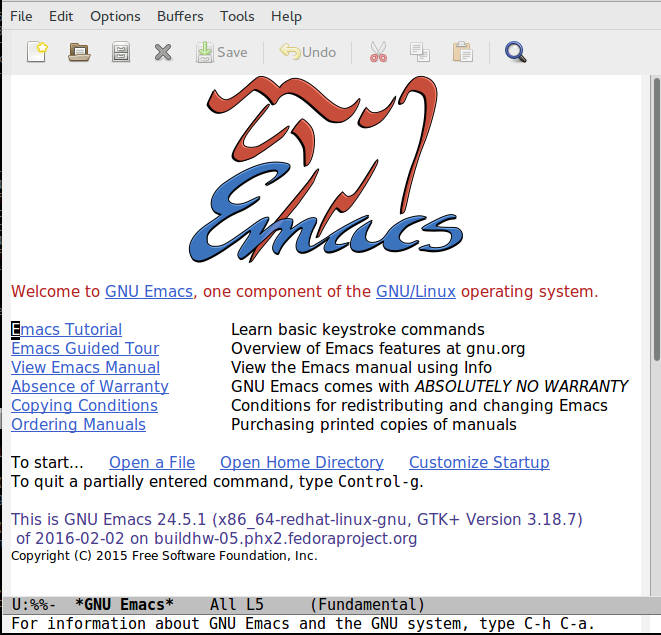
\includegraphics[width=8cm]{figures/emacs_welcome}
\caption{emacs Welcome Screen}
\label{emacsWelcomeScreen}
\end{figure}


So, at the Welcome Screen, you type \tbi{CTRL+h, release the keys and then type i}. You will get the next screen.

\begin{figure}[H]
\centering
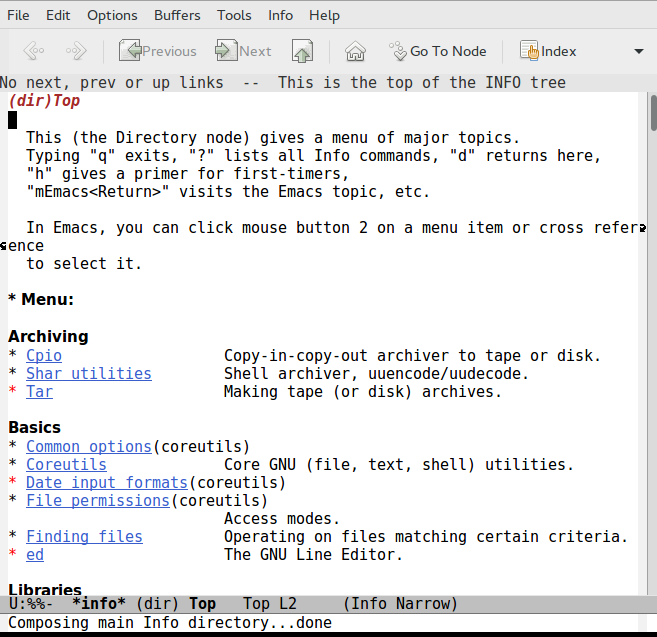
\includegraphics[width=8cm]{figures/emacs_listofinfocmds}
\caption{emacs info command list}
\label{emacsInfoCommandList}
\end{figure}

Now, we need to search for our command. We could just scroll down, but that is time consuming. Let's search for the \tbi{stat} command. Type: CTRL+s to start the search and then type: * (stat)

\begin{figure}[H]
\centering
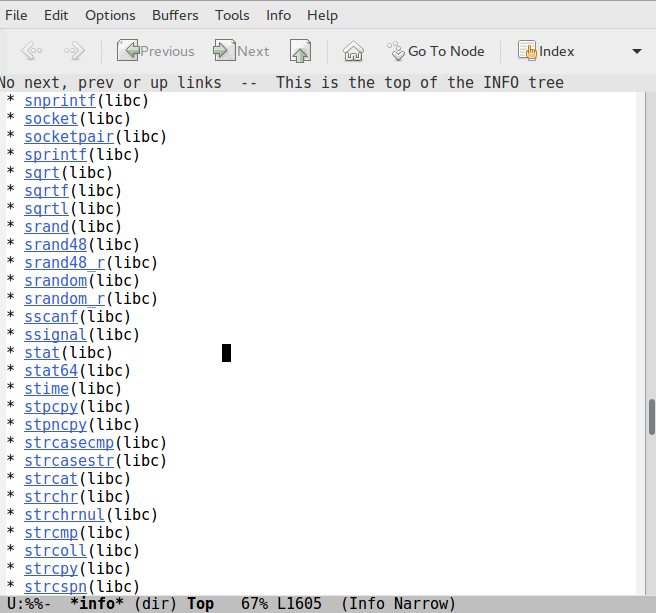
\includegraphics[width=8cm]{figures/emacs_statlist}
\caption{emacs stat entry in list}
\label{emacsStatList}
\end{figure}

Now, simply click on the \tbi{stat} link and the info page opens.

\begin{figure}[H]
\centering
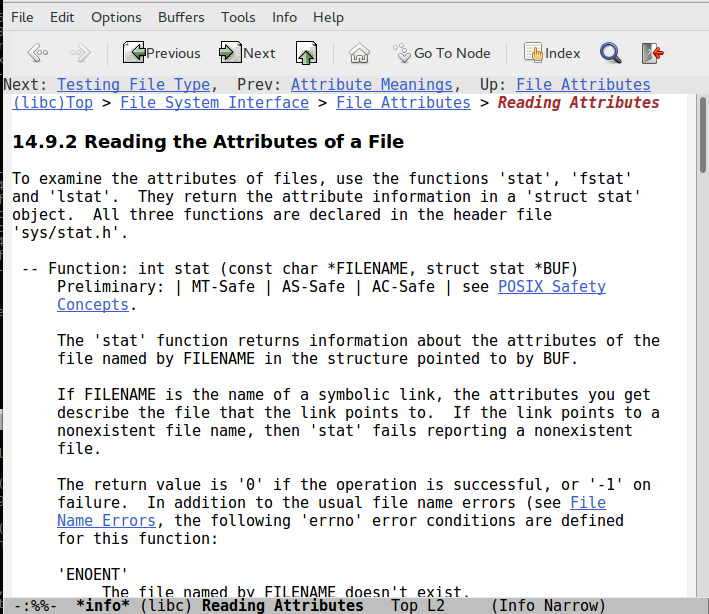
\includegraphics[width=8cm]{figures/emacs_statinfo}
\caption{emacs stat info document}
\label{emacsStatInfo}
\end{figure}

\subsection{coreutils}

Please visit \href{http://www.gnu.org/software/coreutils/coreutils.html}{Coreutils - GNU core utilities}. The following description is provided:

\begin{lstlisting}
The GNU Core Utilities are the basic file, shell and text manipulation utilities of the GNU operating system. These are the core utilities which are expected to exist on every operating system. 
\end{lstlisting}

Any command that is part of the GNU operating system will make reference to the \href{https://www.gnu.org/software/coreutils/manual/coreutils.html#Top}{GNU Coreutils} website. You will find very detailed information on each command.

\begin{lstlisting}[escapeinside={¿}{¿},frame=single,breaklines]
#
# Again, I use ¿\color[rgb]{0.133,0.545,0.133}\latex¿ to add the live hyperlink.
#
¿\tld¿ man ls | grep -A5 "SEE ALSO"
SEE ALSO
Full documentation at: <¿\href{http://www.gnu.org/software/coreutils/ls}{http://www.gnu.org/software/coreutils/ls}¿>
or available locally via: info '(coreutils) ls invocation'
\end{lstlisting}

\subsection{Developers Home Page}

Open source developers typically provide a man page. In one of the previous sections we installed the \keyword{lv} package . Note, the man page provides a link to the developer website.

\begin{lstlisting}[escapeinside={¿}{¿},frame=single,breaklines]
#
# Wouldn't it be nice if manpages had live hyperlinks?  ¿\color[rgb]{0.133,0.545,0.133}\emph{Brush up on your Japanese before clicking this link.}¿
#
¿\tld¿ man lv | grep -A5 "SEE ALSO"
SEE ALSO
LV Homepage: ¿\href{http://www.ff.iij4u.or.jp/\textasciicircum{}nrt/lv/}{http://www.ff.iij4u.or.jp/\ttbb{}nrt/lv/}¿

COPYRIGHT
All rights reserved. Copyright (C) 1996-2004 by NARITA Tomio.
\end{lstlisting}

\subsection{Searching all local resources for best information}

So, we have a number of ways of getting information on a particular command. Let's explore using \keyword{sed}. Note, we are only looking for a reference to the -e option. We may have to open the full man page or the full info document if the information is too cryptic to be helpful and then search inside the full document.

\begin{lstlisting}[escapeinside={¿}{¿},frame=single,breaklines]
#
# Suppose we know that sed has a -e option, but we forgot what that option actually did.
#
# 1. We could use my m- function. I use grep's -w, word option for an exact match. My function is very concise. It just says, yes there is a -e option.
#
¿\tld¿ m- sed | grep -w \\-e
-e script, --expression=script
#
# What about the man page? Note, I added grep's 'after lines of context' option, -A2. Well, this is a bit more helpful.
#
¿\tld¿ man sed | grep -A2 -w \\-e 
	-e script, --expression=script

	add the script to the commands to be executed
--
	If no -e, --expression, -f, or --file option is given, then the first non-option argument is taken  as  the sed  script  to  interpret.  All remaining arguments are names of input files; if no input files are specified, then the standard input is read.
--
	The comment extends until the next newline (or the end of a -e script fragment).

 }  The closing bracket of a { } block.
#
# How about the builtin --help function? Ok, that info is fairly similar to the man page info.
#
¿\tld¿ sed --help | grep -A3 -w \\-e
  -e script, --expression=script
				add the script to the commands to be executed
  -f script-file, --file=script-file
				add the contents of script-file to the commands to be executed
--
If no -e, --expression, -f, or --file option is given, then the first
non-option argument is taken as the sed script to interpret.  All
remaining arguments are names of input files; if no input files are
specified, then the standard input is read.
#
# Alright, let's try the info document? There is a ton of information. I only show a part of the output. As you can see, info really is the full documentation. I only show a small portion of the output. And, yes those backticks are correct...documentation that needs editing by the maintainer!
#
¿\tld¿ info sed | grep -C5 -w \\-e

If you do not specify INPUTFILE, or if INPUTFILE is `-', `sed'
filters the contents of the standard input.  The SCRIPT is actually the
first non-option parameter, which `sed' specially considers a script
and not an input file if (and only if) none of the other OPTIONS
specifies a script to be executed, that is if neither of the `-e' and
`-f' options is specified.

`sed' may be invoked with the following command-line options:

`--version'
--
By default, `sed' prints out the pattern space at the end of each
cycle through the script (*note How `sed' works: Execution Cycle.).
These options disable this automatic printing, and `sed' only
produces output when explicitly told to via the `p' command.

`-e SCRIPT'
`--expression=SCRIPT'
Add the commands in SCRIPT to the set of commands to be run while
processing the input.
.
.
\end{lstlisting}

So, what method should you use? It really depends on what you are looking for. I would suggest that you start with the simplest method and go to the more complex. 

\begin{enumerate}
	\item{my m- function}
	\item{-{}-{}help bash builtin command}
	\item{man page}
	\item{info document}
	\item{external resources on the web}	
\end{enumerate}

\section{Viewing man pages as html}

\subsection{TkMan}

\tbi{TkMan} is an open source package available at \href{https://sourceforge.net/projects/tkman/}{sourceforge}. Here is its description...

\begin{lstlisting}
TkMan is a graphical, hypertext manual page and Texinfo browser for UNIX.
TkMan boasts hypertext links, high quality display and a superior navigational interface,
full text search and much more.
\end{lstlisting}

\subsection{Searching online for manpages}

\begin{enumerate}
	\item{\href{http://grisha.biz/cgi-bin/man}{CentOS Man Pages}}
	\item{\href{http://linuxmanpages.net/index.html}{fedora manuals}}
\end{enumerate}

\subsection{Create a BROWSER environment variable}

\begin{lstlisting}[escapeinside={¿}{¿},frame=single,breaklines]
#
# You can also add this export statement to your .bashrc file.
#
¿\tld¿ export BROWSER=firefox
#
# Add the --html option and Firefox opens the ps manpage as an html document.
#
¿\tld¿ man --html ps
#
# This export statement can be added to your .bashrc file so that it is always available.
#
# We can also create an alias for this command: mh = man --html $1. We would then call it with: mh sed.
#
\end{lstlisting}

\section{Printing a man page}

\subsection{Creating a PDF}

\begin{lstlisting}[escapeinside={¿}{¿},frame=single,breaklines]
#
# First, using the man command itself, create a .ps, post script document.
#
¿\tld¿ man -t stat > stat.ps
#
# If you want to view the actual contents of stat.ps , issue the following command...
#
¿\tld¿ psnup stat.ps
%!PS-Adobe-3.0
%%Creator: groff version 1.22.3
%%CreationDate: Tue Mar 22 15:10:56 2016
%%DocumentNeededResources: font Times-Roman
.
.
%%Trailer
end
%%EOF
Wrote 2 pages, 14536 bytes
\end{lstlisting}

Now that you have a Post Script version of the manpage, open the file with a PDF reader such as the \href{https://help.gnome.org/users/evince/stable/}{Evince Document Viewer}.

\begin{figure}[H]
\centering
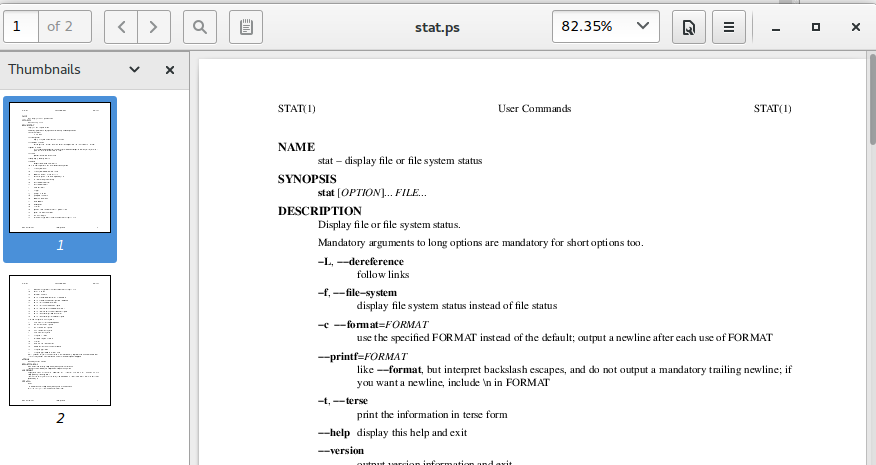
\includegraphics[width=12cm]{figures/statps}
\caption{stat Post Script}
\label{statPS}
\end{figure}

Now, all we have to do is CTRL+p to bring up the print controls. I assume that you have a local or network printer installed. This method allows you to view the man page as a PDF.\\

\subsection{Printing from the command line}

This is the easiet way to print a properly formatted man page.

\begin{lstlisting}[escapeinside={¿}{¿},frame=single,breaklines]
#
# Immediately print the texinfo manpage from the command line.
#
¿\tld¿ man -t texinfo | lpr -pPrinter
#
# Do you like this command? Add it to .bashrc. I will display the function that I added to .bashrc using the type command.  Add all the lines except the first to .bashrc. The type command adds the optional ; character. I did not  enter these when inputing the lines into .bashrc. So, type tells us 'best practices' for writing bash code.
#
¿\tld¿ type pman
pman is a function
pman () 
{ 
while [ $¿\#¿ -ne 0 ]; do
man -t $1 | lpr -pPrinter;
shift;
done
}
#
# Here is how these lines appear in my .bashrc file.
#
¿\tld¿ grep pman -A7 .bashrc
function pman ()
{
while [ $¿\#¿ -ne 0 ]
do
man -t $1 | lpr -pPrinter
shift
done
}
#
# Since the function reads all arguments supplied, we can print several man pages at once. The following command will print the texinfo and printf manpages.
#
¿\tld¿ pman texinfo printf
\end{lstlisting}
